\documentclass{itkmitlproject}

\usepackage{afterpage}
\usepackage{graphicx,amsmath,latexsym,amssymb,amsthm}
\usepackage{indentfirst}
\usepackage{hyperref}
\usepackage{hyphenat}
\usepackage[numbers,square]{natbib}
\usepackage{lipsum}

% \useEnglish
\useThai

\graphicspath{ {images/} }

%1. Your thesis title (THAI)
\newcommand{\ThesisTitle}{สื่อการเรียนรู้การคิดเชิงคำนวณ ในรูปแบบของการเขียนโปรแกรมแบบจับต้องได้}
%2. Your thesis title (ENG)
\newcommand{\ThesisTitleENG}{Learning media for computational thinking in a form of tangible programming}
%3. Author name
\newcommand{\Author}{ภาสวิชญ์ ริ้วทอง}
%4. Author name ENG
\newcommand{\AuthorENG}{Passawit Riewthong}
%5. Author student ID
\newcommand{\SId}{60070073}
%6. Author 2 name
\newcommand{\AuthorTwo}{มารีน่า หนูรามัญ}
%7. Author 2 name ENG
\newcommand{\AuthorTwoENG}{Mareena Nuramun}
%8. Author 2 student ID
\newcommand{\SIdTwo}{60070076}
%9. Advisor name
\newcommand{\Advisor}{รศ.ดร.ปานวิทย์ ธุวะนุติ}
%10. Advisor name ENG
\newcommand{\AdvisorENG}{Assoc. Prof. Dr. Panwit Tuwanut}
%11. ภาคเรียนที่
\newcommand{\Sem}{1}
%12. ปีการศึกษา พ.ศ.
\newcommand{\AcaY}{2563}
%13. ปีการศึกษา ค.ศ.
\newcommand{\AcaYAD}{2020}
%14. วันส่งรายงาน
\newcommand{\SubD}{1 ตุลาคม พ.ศ. 2562}
%15. Copyright year (AD)
\newcommand{\CopyrightYAD}{2020}

\begin{document}
    \frontmatter
    \lhead{}\rhead{}\chead{}\lfoot{}\cfoot{\thepage}\rfoot{}
    \makecover
    \makeinnercover
    \makeengcover
    \makecopyrightcover
    \makethesiscert
    \makeprojectcert

    % Setting margin for page numbering on frontmatter
    \newgeometry{top=1in, bottom=1in, left=1.5in, right=1in, includefoot}
    \setcounter{page}{1}
    \pagenumbering{Roman}

    \makeabstract{
        ทักษะการคิดเชิงคำนวณเป็นทักษะหนึ่งที่เข้ามามีความสำคัญ และเป็นพื้นฐานที่จะนำไปสู่การแก้ไขปัญหาที่ซับซ้อนอย่างเป็นขั้นตอน และมีประสิทธิภาพ
        ด้วยเหตุนี้การเรียนการสอนสำหรับเด็กปฐมวัยในปัจจุบันจึงเริ่มมีการสอดแทรก การสอนทักษะการคิดเชิงคำนวณ ทักษะการคิดวิเคราะห์ในรูปแบบต่าง ๆ
        เพื่อให้เด็ก และเยาวชนสามารถนำเอาทักษะเหล่านี้ไปประยุกต์ใช้กับการแก้ปัญหาในชีวิตประจำวัน รวมถึงต่อไปในอนาคตโดยเฉพาะในยุคที่เทคโนโลยีมีบทบาทมากขึ้นในทุก ๆ ด้าน

        งานวิจัยนี้คณะผู้จัดทำได้ศึกษาพบว่าวิธีการใช้สื่อการเรียนรู้ เช่น หุ่นยนต์ แผนที่แบบตาราง และสิ่งของที่จับต้องได้ อาทิ บล็อก นั้นมีประสิทธิภาพต่อพัฒนาการการเรียนรู้ของเด็กเป็นอย่างมาก
        แต่ในทางกลับกัน สื่อการเรียนรู้การคิดเชิงคำนวณที่มีอยู่ในปัจจุบันมีมูลค่าซื้อขายค่อนข้างสูง ส่งผลให้เด็ก และเยาวชนที่ครอบครัวมีรายได้น้อยสามารถเข้าถึงอุปกรณ์เหล่านี้ได้ยาก
        โดยงานวิจัยนี้มีการพัฒนาอุปกรณ์ Microcontroller เพื่อใช้สำหรับเป็นต้นแบบสื่อการเรียนรู้การคิดเชิงคำนวณ สำหรับเด็ก และเยาวชนในรูปแบบของการเขียนโปรแกรมแบบจับต้องได้
        ด้วยอุปกรณ์ที่ราคาประหยัด ซึ่งสื่อการเรียนรู้นี้จะช่วยพัฒนาทักษะการคิดเชิงคำนวณ และส่งเสริมให้เยาวชนมีการทำกิจกรรมร่วมกันผ่านการคิดวิเคราะห์ และแก้ไขปัญหาตามรูปแบบการเล่นที่กำหนดให้
    }

    \makeabstracteng{
        Computational thinking becomes an essential and fundamental skill that can lead to an effective problem-solving process. Accordingly, several teaching patterns of computational thinking and critical thinking skills were integrated into the current teaching and learning for preschool to enhance children and young people to apply them to solve daily life problems and later, especially in an age where technology is becoming increasingly important.
    }

    \makeack

    \newpage
    \addcontentsline{toc}{chapter}{\contentsname}
    \tableofcontents

    \newpage
    \addcontentsline{toc}{chapter}{\listtablename}
    \listoftables

    \newpage
    \addcontentsline{toc}{chapter}{\listfigurename}
    \listoffigures

    % Reset frontmatter page numbering margin, back to original margin from class file
    \restoregeometry

    \mainmatter
    \lhead{}\rhead{\thepage}\chead{}\lfoot{}\cfoot{}\rfoot{}

    \chapter{บทนำ}
\label{chapter:introduction}

\section{แนวคิด ที่มา และความสำคัญ}
ภาษาคอมพิวเตอร์หรือ Coding เข้ามามีบทบาทสำคัญในช่วงที่เทคโนโลยีมีการเปลี่ยนแปลงอย่างก้าวกระโดด โดยเฉพาะอย่างยิ่งในส่วนของภาคธุรกิจที่เริ่มมีการนำเทคโนโลยีมาปรับใช้ทั้งภายใน และภายนอกองค์กรเพิ่มมากขึ้น
ส่งผลให้อัตราการจ้างงานในรูปแบบของบุคลากรลดลงในหลายแผนก โดยเฉพาะแผนกที่เทคโนโลยีสามารถทำงานได้มีประสิทธิภาพกว่าการใช้ทรัพยากรมนุษย์ แต่ในทางตรงกันข้ามบริษัทเบื้องหลังที่ผลิตเทคโนโลยีต่าง ๆ
กลับมีแนวโน้มในการเพิ่มบุคลากรทางคอมพิวเตอร์เพื่อพัฒนา และเพิ่มกำลังการผลิตเทคโนโลยี ให้ตอบสนองต่อความต้องการของหลายภาคส่วน ด้วยเหตุนั้น ภาษาคอมพิวเตอร์จึงเริ่มเข้ามาเป็นพื้นฐานของระบบการศึกษาของเด็กในศตวรรษที่ 21
เพื่อเสริมสร้างทักษะการคิดวิเคราะห์ และฝึกฝนกระบวนการคิดอย่างเป็นเหตุเป็นผล ซึ่งเป็นสิ่งที่จำเป็นอย่างยิ่งสำหรับการดำเนินชีวิตในปัจจุบัน และต่อไปในอนาคต

กระนั้น การเข้าถึงภาษาคอมพิวเตอร์ทางตรงยังมีข้อจำกัดหลายอย่างทั้งด้านอุปกรณ์ หรือ บุคลากรทางการศึกษาที่มีอย่างจำกัด ซึ่งทำให้การศึกษาภาษาคอมพิวเตอร์ยังคงเป็นไปได้ยาก
ทางผู้จัดทำจึงได้เล็งเห็นถึงแนวทางในการนำความรู้ด้านการคิดเชิงคำนวณ \cite{KnowComputationalThinking} (Computational Thinking \cite{IntroductionToComputationalThinking}) ที่ประกอบไปด้วย 4 แนวคิด ดังนี้
\begin{enumerate}
    \item การแบ่งย่อยปัญหา (Decomposition)
    \item การเข้าใจรูปแบบ (Pattern Recognition)
    \item ความคิดเชิงนามธรรม (Abstraction)
    \item การออกแบบขั้นตอนวิธี (Algorithm Design)
\end{enumerate}
ซึ่งเป็นพื้นฐานของการเรียนรู้ภาษาคอมพิวเตอร์มาพัฒนาเป็นสื่อการเรียนรู้ในรูปแบบของการเขียนโปรแกรมแบบจับต้องได้ เพื่อให้เด็ก และเยาวชน สามารถเรียนรู้ เข้าใจ
และเข้าถึงทักษะการคิดเชิงคำนวณ และทักษะการคิดวิเคราะห์ อีกทั้งผู้จัดทำยังต้องการที่จะลดปัญหาสายตาในเด็กที่อาจเกิดจากการทำกิจกรรมหน้าจอคอมพิวเตอร์เป็นเวลานาน
(ซึ่งหากเป็นการเรียนรู้การเขียนภาษาคอมพิวเตอร์รูปแบบเดิมส่วนใหญ่จะต้องทำผ่านคอมพิวเตอร์เป็นหลัก) โดยการพัฒนาอุปกรณ์ Microcontroller
เพื่อใช้สำหรับเป็นต้นแบบสื่อการเรียนรู้การคิดเชิงคำนวณที่เหมาะกับเด็ก และเยาวชนในรูปแบบการเขียนโปรแกรมแบบจับต้องได้ ซึ่งอุปกรณ์นี้จะไม่มีการใช้หน้าจอทุกชนิด
โดยจะทดแทนด้วยหุ่นยนต์ การ์ด และแผนที่ที่มีการออกแบบมาเพื่อเด็ก และเยาวชนโดยเฉพาะ นอกจากนั้นยังอาศัยอุปกรณ์ที่มีราคาไม่แพง รวมถึงมีวิธีการสร้างที่ไม่ซับซ้อนซึ่งเหมาะกับการผลิตเพื่อใช้งานเองของโรงเรียน องค์กร หรือบุคคลทั่วไป

\section{วัตถุประสงค์ของโครงงาน}
\begin{enumerate}
    \item พัฒนาสื่อการเรียนรู้ทักษะการคิดวิเคราะห์ และการแก้ปัญหา ในรูปแบบของการเขียนโปรแกรมแบบจับต้องได้ ที่เหมาะสมสำหรับเด็ก และเยาวชนในแต่ละช่วงอายุ
    \item ส่งเสริมการเรียนการสอนทักษะการคิดวิเคราะห์ และการแก้ปัญหา โดยเริ่มตั้งแต่ระดับประถมศึกษาขึ้นไป 
    \item สร้างแรงจูงใจแก่เด็ก และเยาวชน ในการพัฒนาทักษะการคิดวิเคราะห์ และการแก้ปัญหาอย่างเป็นขั้นตอน
\end{enumerate}

\section{ขอบเขตการดำเนินงาน}
พัฒนาอุปกรณ์ Microcontroller เพื่อใช้สำหรับเป็นสื่อการเรียนรู้การคิดเชิงคำณวณ สำหรับเด็ก และเยาวชนที่อายุตั้งแต่ 7 ปีขึ้นไป ด้วยอุปกรณ์ที่สามารถจัดหาได้ง่าย ราคาถูก
โดยจะทำให้ชิ้นส่วนอื่นที่นอกเหนือจากตัว Microcontroller มีลักษณะที่เข้าใจง่าย และส่งเสริมพัฒนาการด้านการคิดวิเคราะห์ของเด็กโดยเฉพาะ ประกอบไปด้วย
การ์ดที่อยู่ในรูปแบบของจิ๊กซอว์ และแผนที่ตาราง รวมไปถึงการจัดทำคู่มือผู้ใช้ และวิธีการติดตั้งที่เข้าใจง่ายรองรับการเป็น Opensource สำหรับผู้ปกครอง หรือโรงเรียนที่สนใจนำไปเป็นสื่อการเรียนรู้ให้เด็ก และเยาวชน

\section{ขั้นตอนการดำเนินงาน}
\begin{enumerate}
    \item กำหนด และวิเคราะห์ปัญหา
    \item ศึกษาทฤษฎี และหลักการของการคิดเชิงคำนวณ
    \item ศึกษาพัฒนาการด้านการเรียนรู้ของเด็ก และเยาวชนที่มีอายุตั้งแต่ 7 ปีขึ้นไป
    \item ศึกษาอุปกรณ์ และเทคโนโลยีที่เกี่ยวข้องกับการพัฒนาสื่อการเรียนรู้สำหรับเด็ก
    \item ออกแบบสื่อการเรียนรู้
    \item พัฒนาต้นแบบสื่อการเรียนรู้
    \item ทดสอบ และปรับปรุง
    \item จัดทำคู่มือสำหรับผู้ใช้
    \item สรุปผลการพัฒนา
    
\end{enumerate}

\section{ประโยชน์ที่คาดว่าจะได้รับ}
\begin{enumerate}
    \item เพิ่มประสิทธิภาพการเรียนรู้ทักษะการคิดเชิงคำนวณ ซึ่งเป็นพื้นฐานของการเขียนโปรแกรม ให้แก่เด็ก และเยาวชน
    \item เด็ก และเยาวชน สามาถพัฒนาทักษะการคิดเชิงคำนวณได้อย่างทั่วถึง
    \item สนับสนุนเด็ก เยาวชน และบุคคลทั่วไป ที่มีความสนใจ และต้องการฝึกฝนทักษะการคิดเชิงคำนวณ
    
\end{enumerate}
    \chapter{ทฤษฎี และเทคโนโลยีที่เกี่ยวข้อง}
\label{chapter:literature-review}

\section{ทฤษฎี และงานวิจัยที่เกี่ยวข้อง}
\subsection{การคิดเชิงคำนวณ (Computational Thinking)}
การคิดเชิงคำนวณคือกระบวนการแก้ไขปัญหาโดยทำการวิเคราะห์ ตีความ และทำความเข้าใจปัญหา แบ่งย่อยปัญหาที่ซับซ้อนให้ออกมาเป็นหลาย ๆ ส่วน และทำการแก้ปัญหาแบบเป็นขั้นตอน

Jeannette M. Wing นักวิจัยด้านวิทยาการคอมพิวเตอร์ กล่าวว่า การคิดเชิงคำนวณเกี่ยวข้องกับการแก้ไขปัญหา การออกแบบระบบ และการทำความเข้าใจพฤติกรรมของมนุษย์โดยอาศัยแนวคิดพื้นฐานของวิทยาการคอมพิวเตอร์ \cite{ComputationalThinking} โดยการคิดเชิงคำนวณนั้นประกอบไปด้วย 4 แนวคิดสำคัญ ได้แก่
\begin{enumerate}
    \item การแบ่งย่อยปัญหา (Decomposition) แบ่งปัญหาที่มีความซับซ้อนออกเป็นหลาย ๆ ส่วนเพื่อให้ง่ายต่อการจัดการแก้ปัญหานั้น
    \item การเข้าใจรูปแบบ (Pattern Recognition) หารูปแบบที่เหมือนหรือคล้ายกันของแต่ละปัญหาที่เคยเกิดขึ้น
    \item ความคิดเชิงนามธรรม (Abstraction) สามารถระบุถึงปัญหาหลักหรือปัญหาที่เกี่ยวข้องได้
    \item การออกแบบขั้นตอนวิธี (Algorithm Design) ออกแบบ และพัฒนาขั้นตอนของการแก้ไขปัญหา
\end{enumerate}
โดยแต่ละแนวคิดนั้นมีความสำคัญเป็นอย่างมาก หากขาดแนวคิดใดไป การแก้ปัญหาแบบการคิดเชิงคำนวณมักจะเกิดความติดขัด และต้องกลับไปเริ่มต้นกระบวนการใหม่ตั้งแต่แนวคิดแรกอีกครั้ง

\subsection{สุขภาพตากับเด็กยุคดิจิตอล}
จากบทความของโรงพยาบาลบํารุงราษฎร์ ซึ่งมีการศึกษาเกี่ยวกับสิ่งที่ส่งผลต่อสายตาของเด็กที่มีการใช้โทรศัพท์มือถือ แทบเล็ต และหน้าจอต่าง ๆ เป็นเวลานาน
พบว่าสิ่งเหล่านี้อาจมีส่วนทำให้เกิดปัญหาสายตาในเด็กเช่น สายตาสั้น สายตาเอียง ตาแพ้แสงได้ โดยตัวอย่างปัจจัยที่ทำให้เด็กสายตาสั้นเพิ่มขึ้น ได้แก่
\begin{itemize}
    \item พันธุกรรม หากเด็กมีบุคคลในครอบครัวที่มีปัญหาสายตา เช่น สายตาสั้น สายตาเอียง ก็เป็นปัจจัยหนึ่งที่ทำให้เด็กเกิดปัญหาสายตาได้
    \item การทำกิจกรรมที่มีการใช้สายตาระยะใกล้เป็นเวลานาน ซึ่งรวมไปถึงการใช้อุปกรณ์คอมพิวเตอร์ และโทรศัพท์มือถือ
    \item ผู้ที่มีการทำกิจกรรมกลางแจ้งน้อย เนื่องจากมีการศึกษาที่กล่าวว่าวิตามินดีในแสงแดดเป็นปัจจัยที่ดีในการช่วยชะลอภาวะสายตาสั้นในเด็ก \cite{ChildrenEyesHealthCare}
\end{itemize}
และภายในบทความยังมีการกล่าวถึงอาการ Computer Vision Syndrome (CVS) หรือภาวะที่เกิดจากการใช้สายตากับคอมพิวเตอร์เป็นเวลานานโดยความรุนแรงจะเพิ่มขึ้นตามระยะเวลาในการใช้งาน
และจ้องหน้าจอคอมพิวเตอร์อย่างต่อเนื่อง ซึ่งผลกระทบที่ตามมาจากภาวะนี้เช่น ปวดเมื่อยตา ตาแห้ง แสบตา เคืองตา แพ้แสง เป็นต้น \cite{ComputerVisionSyndrome}

\subsection{แนวคิด CS Unplugged}
CS Unplugged หรือ Computer Science Unplugged คือแนวคิดการเรียนการสอนด้านคอมพิวเตอร์สำหรับเด็กอนุบาลจนถึงชั้นประถมปลายที่มุ่งเน้นการสร้างความเข้าใจพื้นฐานของวิทยาศาสตร์คอมพิวเตอร์
และตรรกศาสตร์ผ่านการทำกิจกรรมต่าง ๆ โดยไม่ใช้คอมพิวเตอร์ เช่น เกมกระดาน บัตรคำ การ์ด หรืออุปกรณ์ต่าง ๆ ที่มีอยู่รอบตัว \cite{CSUnplugged} \cite{CSUnplugged2}

CS Unplugged นั้นเริ่มมาจากกลุ่มนักวิทยาศาสตร์ด้านคอมพิวเตอร์ชาวนิวซีแลนด์ 3 คนคือ Tim Bell กับ Ian H. Witten และ Mike Fellows ที่ได้ร่วมกันเขียนหนังสือ “Computer Science Unplugged”
ซึ่งมีเนื้อหาเกี่ยวกับกิจกรรมการเรียนรู้ที่ฝึกการคิดวิเคราะห์ และแก้ปัญหาอย่างเป็นระบบโดยไม่ต้องอาศัยการใช้คอมพิวเตอร์ โดยจะเน้นไปที่การมีปฏิสัมพันธ์กับเพื่อนหรือบุคคลในชั้นเรียน สร้างความสนุกสนาน และสอดแทรกสาระไปพร้อม ๆ กัน

ปัจจุบันแนวคิด CS Unplugged ได้รับความนิยมอย่างแพร่หลายไปทั่วโลก และมีการแปลหนังสือ “Computer Science Unplugged” ไปเป็นภาษาต่าง ๆ อีกมากมาย สำหรับภาษาไทยได้รับการแปลโดยอาจารย์
และนักศึกษามหาวิทยาลัยธรรมศาสตร์ในชื่อ “ซีเอส อันปลั๊ก โปรแกรมเสริมสมรรถนะ และขยายความสามารถของเด็กระดับปฐมวัย (ฉบับแปลภาษาไทย)” สามารถดาวน์โหลดหนังสือได้ที่
https://resources.aiat.or.th/cs-unplugged/ หรือสามารถเข้าไปศึกษาเพิ่มเติมเกี่ยวกับแนวคิดนี้ได้ที่ https://csunplugged.org

\begin{figure}[ht]
    \centering
    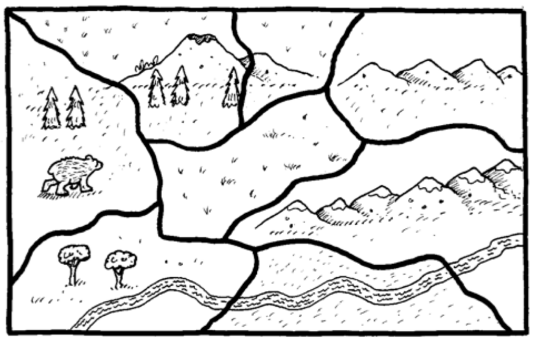
\includegraphics[width=110mm,scale=0.6]{CS-Unplugged.png}
    \caption{ตัวอย่างกิจกรรม CS Unplugged}
    \label{fig:CS-Unplugged}
\end{figure}

\section{เทคโนโลยีที่เกี่ยวข้อง}
\subsection{QR Code (รหัสคิวอาร์) \cite{VarietyOfQRCode}}
QR code มาจากคำว่า Quick Response Code โดย QR code คือบาร์โค้ดประเภท Matrix (หรือบาร์โค้ด 2 มิติ) มีลักษณะเป็นสี่เหลี่ยม ภายในประกอบไปด้วยโมดูลสีดำบนพื้นหลังสีขาว ใช้สำหรับเก็บข้อมูลประเภทข้อความซึ่งประกอบไปด้วยตัวอักษร และตัวเลข โดยในปัจจุบันมีการนำไปประยุกต์ใช้เก็บข้อมูลที่หลากหลาย เช่น ที่อยู่เว็บไซต์ (URL) ข้อความ หรือหมายเลขโทรศัพท์ 

QR code ถูกคิดค้นขึ้นที่ประเทศญี่ปุ่น โดยบริษัทเดนโซ-เวฟ (Denso-Wave) เมื่อปี พ.ศ 2537 มีความแตกต่างจาก Barcode หนึ่งมิติธรรมดาทั่วไปคือมันสามารถเก็บข้อมูลได้ 2 ทิศทาง โดยสามารถเก็บข้อมูลได้ทั้งในรูปแบบแนวตั้งหรือในรูปแบบแนวนอนซึ่งข้อแตกต่างนี้ทำให้ QR code สามารถเก็บข้อมูลได้มากกว่า Barcode หนึ่งมิติถึง 200 เท่า หรือหมายความว่ามันสามารถบรรจุข้อมูลได้มากถึง 4,000 ตัวอักษร และ 7,000 ตัวเลข

โดยการอ่าน QR code นั้นสามารถทำได้ง่าย ๆ โดยการใช้อุปกรณ์ที่มีกล้อง เช่น โทรศัพท์มือถือหรือแท็บเลตที่ได้ทำการติดตั้งโปรแกรมถอดรหัสเอาไว้แสกนไปที่ QR code จากนั้นข้อมูลที่ถูกเข้ารหัสไว้ก็จะแสดงออกมา และในปัจจุบันมี QR code เกิดขึ้นมากมายหลายประเภทจากหลายบริษัทผู้ผลิต ตัวอย่างเช่น
\begin{enumerate}[listparindent=1.25em]
    \item QR Code Model 1 และ QR Code Model 2

    เป็นรูปแบบของ QR Code ที่สามารถเห็นได้ทั่วไป และมีการใช้อย่างแพร่หลายมากที่สุดในขณะนี้ หลักการทำงานของ QR Code ชนิดนี้คือจะมีการใช้ตำแหน่งในการตรวจสอบรูปแบบ (Position detection pattern) 3 ตำแหน่งคือ ซ้ายบน ขวาบน ซ้ายล่างโดย Model 1 เป็น QR Code ตัวต้นแบบ ซึ่งขนาดที่ใหญ่ที่สุดของ Model 1 คือ เวอร์ชั่น 14 (73 x 73 โมดูล) ที่สามารถเก็บข้อมูลชนิดตัวเลขได้สูงสุดถึง 1,167 ตัว 

    Model 2 ได้รับการพัฒนามาจาก Model 1 เพื่อให้ประสิทธิภาพการอ่านดียิ่งขึ้น โดย Model 2 จะอ้างถึงรูปแบบการจัดตำแหน่งที่ฝังอยู่ ทำให้สามารถอ่านได้แม้ตัว QR Code จะผิดเพี้ยนไปจากเดิมก็ตาม โดยขนาดที่ใหญ่ที่สุดของ Model 2 คือ เวอร์ชั่น 40 (177 x 177 โมดูล) ที่สามารถเก็บข้อมูลชนิดตัวเลขได้สูงสุดถึง 7,089 ตัว ซึ่งในปัจจุบัน Model 2 คือรูปแบบที่นิยมมากที่สุด
    \begin{figure}[ht]
        \centering
        
\includegraphics[width=110mm,scale=0.6]{qrcode_model1and2.png}
        \caption{QR Code Model 1 และ QR Code Model 2}
        \label{fig:qrcode_model1and2}
    \end{figure}

    \item Micro QR Code

    Micro QR Code คือ QR Code ที่มีขนาดเล็กกว่า QR Code ปกติ มีการใช้ตำแหน่งในการตรวจสอบรูปแบบ (Position detection pattern) เพียง 1 ตำแหน่ง เพื่อเป็นการลดขนาดของ QR Code โดย Micro QR Code มี 4 เวอร์ชั่น ขนาดเล็กที่สุดคือ 11 x 11 โมดูล และขนาดใหญ่สุดคือ 17 x 17 โมดูลที่สามารถเก็บข้อมูลตัวเลขได้ถึง 35 ตัว นิยมใช้บนบรรจุภัณฑ์ของผลิตภัณฑ์
    \begin{figure}[ht]
        \centering
        
\includegraphics[width=40mm,scale=0.6]{microqr.png}
        \caption{Micro QR Code}
        \label{fig:microqr}
    \end{figure}

    \item iQR Code

    QR Code รูปแบบนี้สามารถผลิตได้ 2 รูปทรงคือแบบสี่เหลี่ยมจัตุรัส และแบบสี่เหลี่ยมผืนผ้า ขนาดใหญ่ที่สุดคือ เวอร์ชั่น 61 (422x422 โมดูล) ซึ่งสามารถเก็บข้อมูลตัวเลขได้ประมาณ 40,000 ตัว โดยมีการออกแบบมาเพื่อให้อ่านง่ายขึ้น และนำไปใช้ในพื้นที่จำกัดได้สะดวกมากยิ่งขึ้น นิยมนำไปใช้บนป้ายกำกับสินค้า
    \begin{figure}[ht]
        \centering
        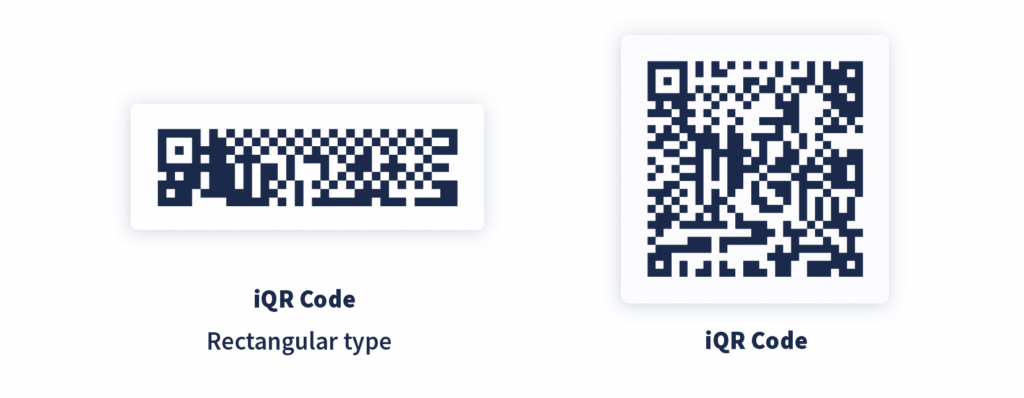
\includegraphics[width=110mm,scale=0.6]{iqrcode.png}
        \caption{iQR Code}
        \label{fig:iqrcode}
    \end{figure}

    \item SQRC Code

    SQRC Code เป็นรูปแบบของ QR Code ที่มีข้อจำกัดในการอ่านข้อมูล กล่าวคือการอ่านข้อมูลจำเป็นต้องใช้กระบวนการที่ซับซ้อนเช่นการเข้ารหัสข้อมูล และการถอดรหัสข้อมูลหลังจากทำการอ่านข้อมูลโดยอุปกรณ์ต่าง ๆ SQRC Code ได้รับการพัฒนาโดยบริษัท Denso-Wave เพื่อให้ง่ายต่อการเข้ารหัส และใช้ข้อมูลที่ไม่เปิดเผยต่อสาธารณะรวมถึงข้อมูลส่วนบุคคล และข้อมูลภายในองค์กร โดยมีรูปลักษณ์ที่เหมือนกับ QR Code ธรรมดาทุกอย่าง แต่สำหรับการอ่านจำเป็นที่จะต้องใช้เครื่องมือเฉพาะ \cite{SQRC}
    \begin{figure}[ht]
        \centering
        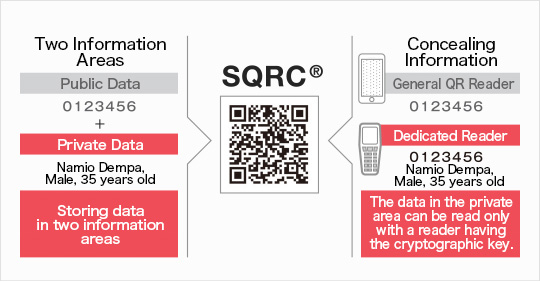
\includegraphics[width=100mm,scale=0.6]{sqrc.jpg}
        \caption{SQRC Code}
        \label{fig:sqrc}
    \end{figure}

    \pagebreak
    \item Frame QR
    
    Frame QR คือ QR Code ที่มีพื้นที่ว่างตรงกลาง (canvas area) ซึ่งสามารถนำรูปหรือตัวอักษรมาใส่ได้ และไม่มีผลต่อการอ่านข้อมูลของ QR Code นิยมนำไปใช้ในการนำเสนอสินค้าหรืออื่น ๆ ได้หลายวัตถุประสงค์
    \begin{figure}[ht]
        \centering
        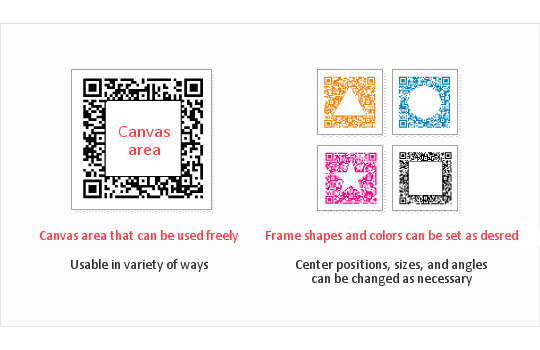
\includegraphics[width=90mm,scale=0.6]{frameqr.jpg}
        \caption{Frame QR}
        \label{fig:frameqr}
    \end{figure}

    \item HCC2D
    
    เป็นรูปแบบของ QR Code ที่ยังอยู่ในขั้นพัฒนาตัวต้นแบบ โดย QR Code ชนิดนี้จะมีการใช้สี CMYK เพื่อเพิ่มปริมาณการเก็บข้อมูล
    \begin{figure}[ht]
        \centering
        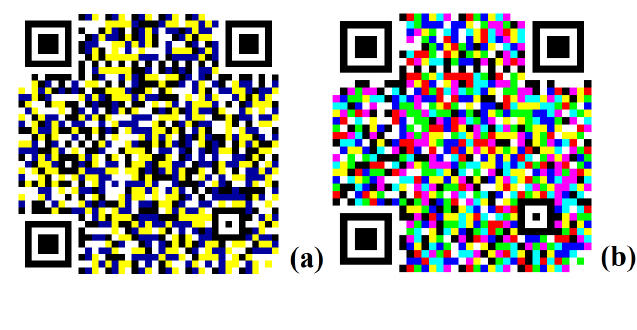
\includegraphics[width=60mm,scale=0.6]{hcc2d.png}
        \caption{HCC2D}
        \label{fig:hcc2d}
    \end{figure}

    \item LogoQ
    
    QR Code แบบใหม่ที่นำเอาโลโก้มารวมกับ QR Code ธรรมดา และนำไปสร้างใหม่ด้วย LogoQ algorithm ซึ่งมีผลลัพท์ที่ได้ตามตัวอย่างในรูปที่ \ref{fig:logoq}
    \begin{figure}[ht]
        \centering
        
\includegraphics[width=100mm,scale=0.6]{logoq.png}
        \caption{LogoQ}
        \label{fig:logoq}
    \end{figure}

\end{enumerate}

\subsection{โมดูล ESP32 CAM}
โมดูลพิเศษซึ่งมาพร้อมกับกล้อง OV2640 ความละเอียด 2 ล้านพิกเซล และ microSD card ในตัว ใช้ชิพ ESP32 ในการเชื่อมต่อกับสัญญาณ Wi-Fi หรือ Bluetooth ที่คลื่นความถี่ 2.4 GHz
ออกแบบด้วยเทคโนโลยี TSMC พลังงานต่ำพิเศษ 40 นาโนเมตร โดย ESP32 CAM นั้น สามารถเป็นได้ทั้งตัวรับสัญญาณ และตัวปล่อยสัญญาณได้ในขณะเดียวกัน แต่ข้อเสียของมันคือไม่มีช่อง micro USB
ไว้สำหรับการอัพโหลด ทำให้ต้องอาศัย USB to TTL ร่วมด้วย \cite{ESP32CAM}
\begin{figure}[ht]
    \centering
    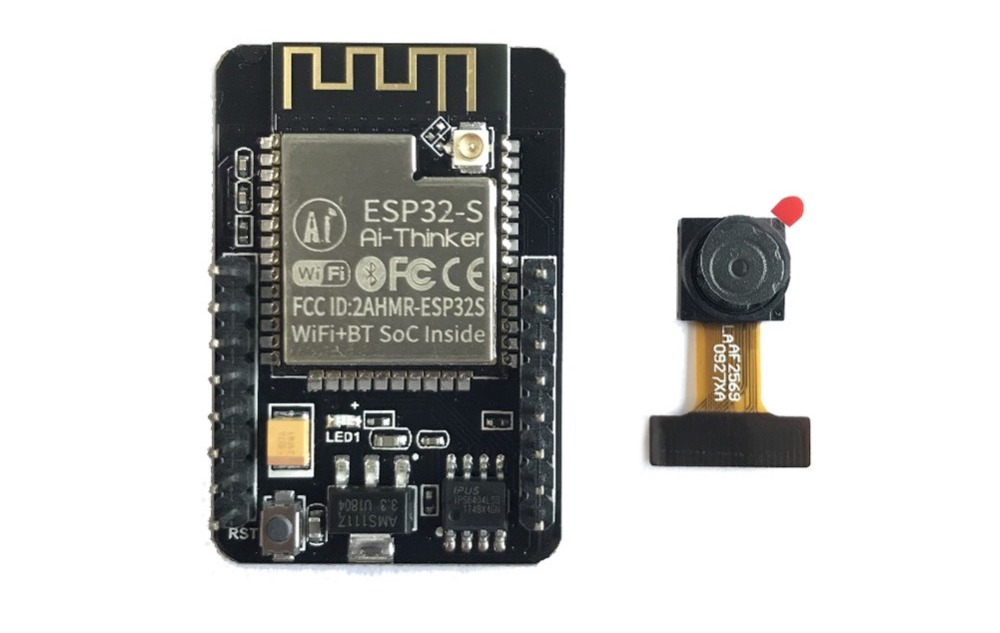
\includegraphics[width=70mm,scale=0.6]{esp32-cam.jpg}
    \caption{ESP32 CAM}
    \label{fig:esp32-cam}
\end{figure}

\subsection{L298N (Motor Driver)}
โมดูลสำหรับจ่ายไฟแบบควบคุมกำลังไฟได้ ซึ่งสามารถจ่ายไฟให้มอเตอร์ 2 ตัวแบบแยกอิสระ โดยใช้วงจร H-Bridge จ่ายไฟเข้ามอเตอร์ตามขั้วที่กำหนดและควบคุมความเร็วด้วยสัญญาณ PWM

\subsection{Gear Motor}
มอเตอร์แม่เหล็กแบบเพลาเดี่ยว โดยหลักการทำงานของ Gear Motor คือการเปลี่ยนพลังงานไฟฟ้าให้หลายเป็นพลังงานกลเพื่อควบคุมรอบการทำงานหรือการหมุนของวัตถุ มีหลายขนาดและรองรับแรงดันไฟฟ้าต่างกัน
\begin{figure}
    \centering
    \begin{minipage}{.5\textwidth}
      \centering
      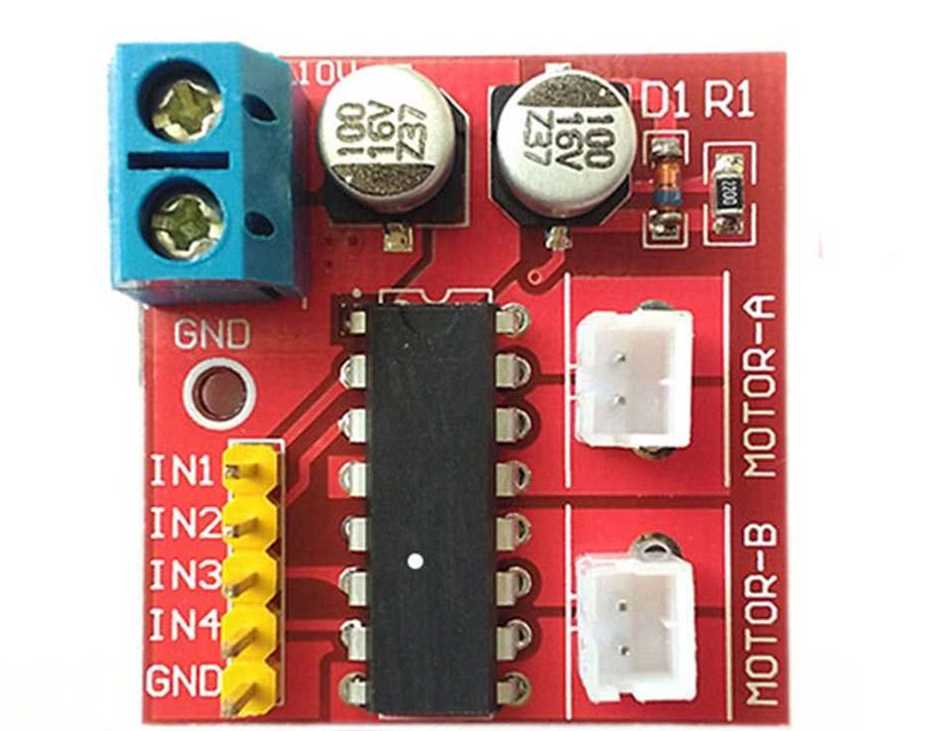
\includegraphics[width=50mm,scale=0.6]{l298n.jpg}
      \caption{Motor Driver}
      \label{fig:l298n}
    \end{minipage}%
    \begin{minipage}{.5\textwidth}
      \centering
      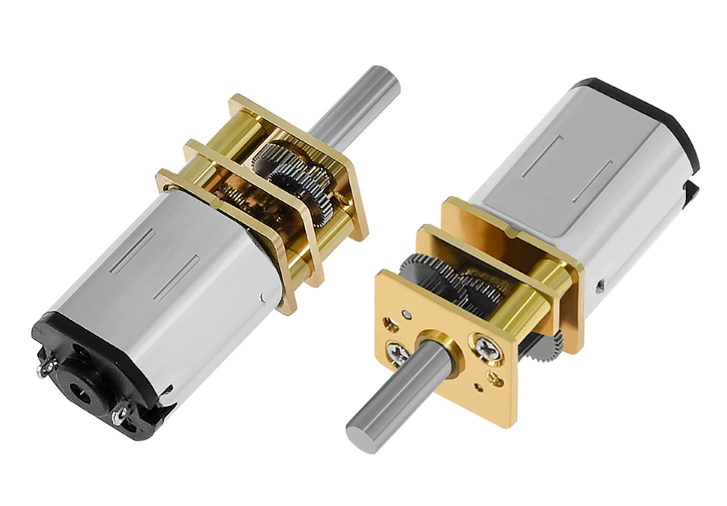
\includegraphics[width=50mm,scale=0.6]{gear-motor.png}
      \caption{Gear Motor}
      \label{fig:gear-motor}
    \end{minipage}
\end{figure}

\subsection{Arduino}

    \chapter{วิธีการดำเนินการวิจัย}
\label{chapter:experiment}

\section{วิเคราะห์ความต้องการ}
\subsection{ความต้องการส่วนหน้าที่หลักของระบบ (Functional Requirement)}
\begin{itemize}
    \itemsep0em
    \item หุ่นยนต์สามารถทำตามชุดคำสั่งจากแผ่นคำสั่งได้
    \item หุ่นยนต์สามารถอ่าน QR Code บนแผ่นคำสั่งได้
\end{itemize}

\subsection{ความต้องการส่วนที่ไม่ใช่หน้าที่หลักของระบบ (Non-functional Requirement)}
\begin{itemize}
    \itemsep0em
    \item ออกแบบอุปกรณ์ให้มีความปลอดภัยต่อการใช้งานของเด็ก
    \item หุ่นยนต์สามารถอ่านข้อมูลจากแผ่นคำสั่งได้ถูกต้อง
    \item ใช้งานง่าย
    \item รองรับการขยายตัวของระบบ
\end{itemize}

\section{การวิเคราะห์และออกแบบระบบ}
\subsection{การออกแบบอุปกรณ์}
สื่อการเรียนรู้การคิดเชิงคำนวณในรูปแบบการเขียนโปรแกรมแบบจับต้องได้พัฒนาขึ้นเพื่อเพิ่มประสิทธิภาพ และสนับสนุนการเรียนรู้ทักษะการคิดเชิงคำนวณแก่เด็ก และเยาวชน ประกอบด้วย 3 ส่วนหลัก คือ หุ่นยนต์เคลื่อนที่ได้ แผ่นคำสั่ง และแผนที่แบบตาราง 

ในส่วนของวัสดุและอุปกรณ์สำหรับทำตัวหุ่นยนต์จะมีความปลอดภัยและมีรูปลักษณ์ที่เหมาะสำหรับการใช้งานของเด็ก เพิ่มความปลอดภัยด้วยการใช้วัสดุที่เป็น Food Grade และรูปทรงที่ไม่เป็นอันตรายต่อการใช้งานด้วยการออกแบบให้มีส่วนโค้งเพื่อลดความแหลมคม
\begin{figure}[ht]
    \centering
    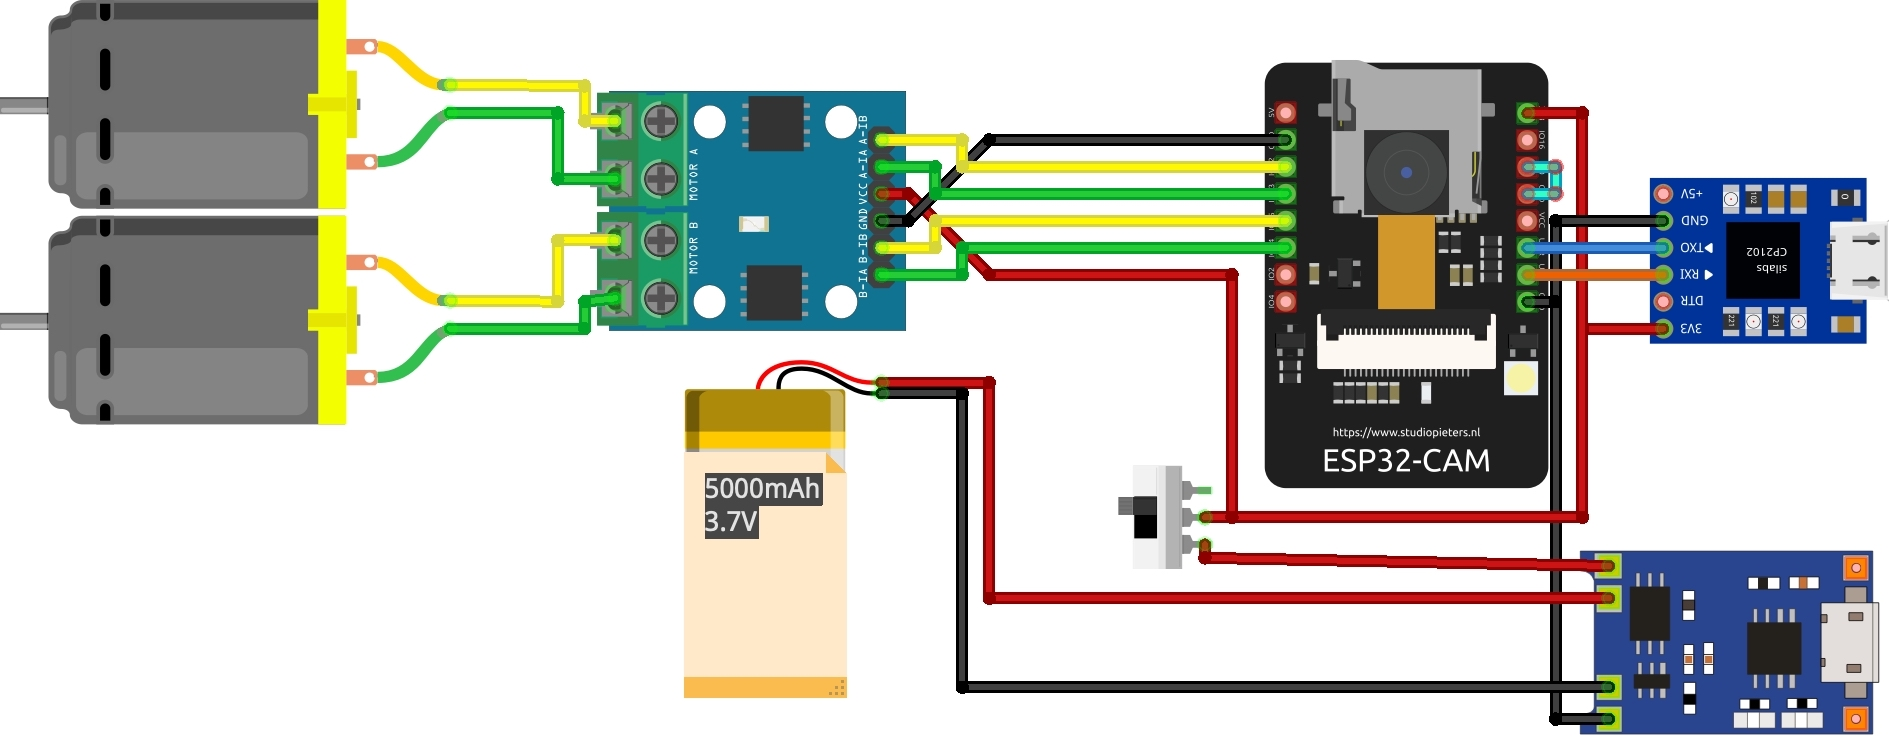
\includegraphics[width=120mm,scale=0.6]{circuit _sketch.jpg}
    \caption{การออกแบบวงจร}
    \label{fig:circuit}
\end{figure}

\begin{figure}[ht]
    \centering
    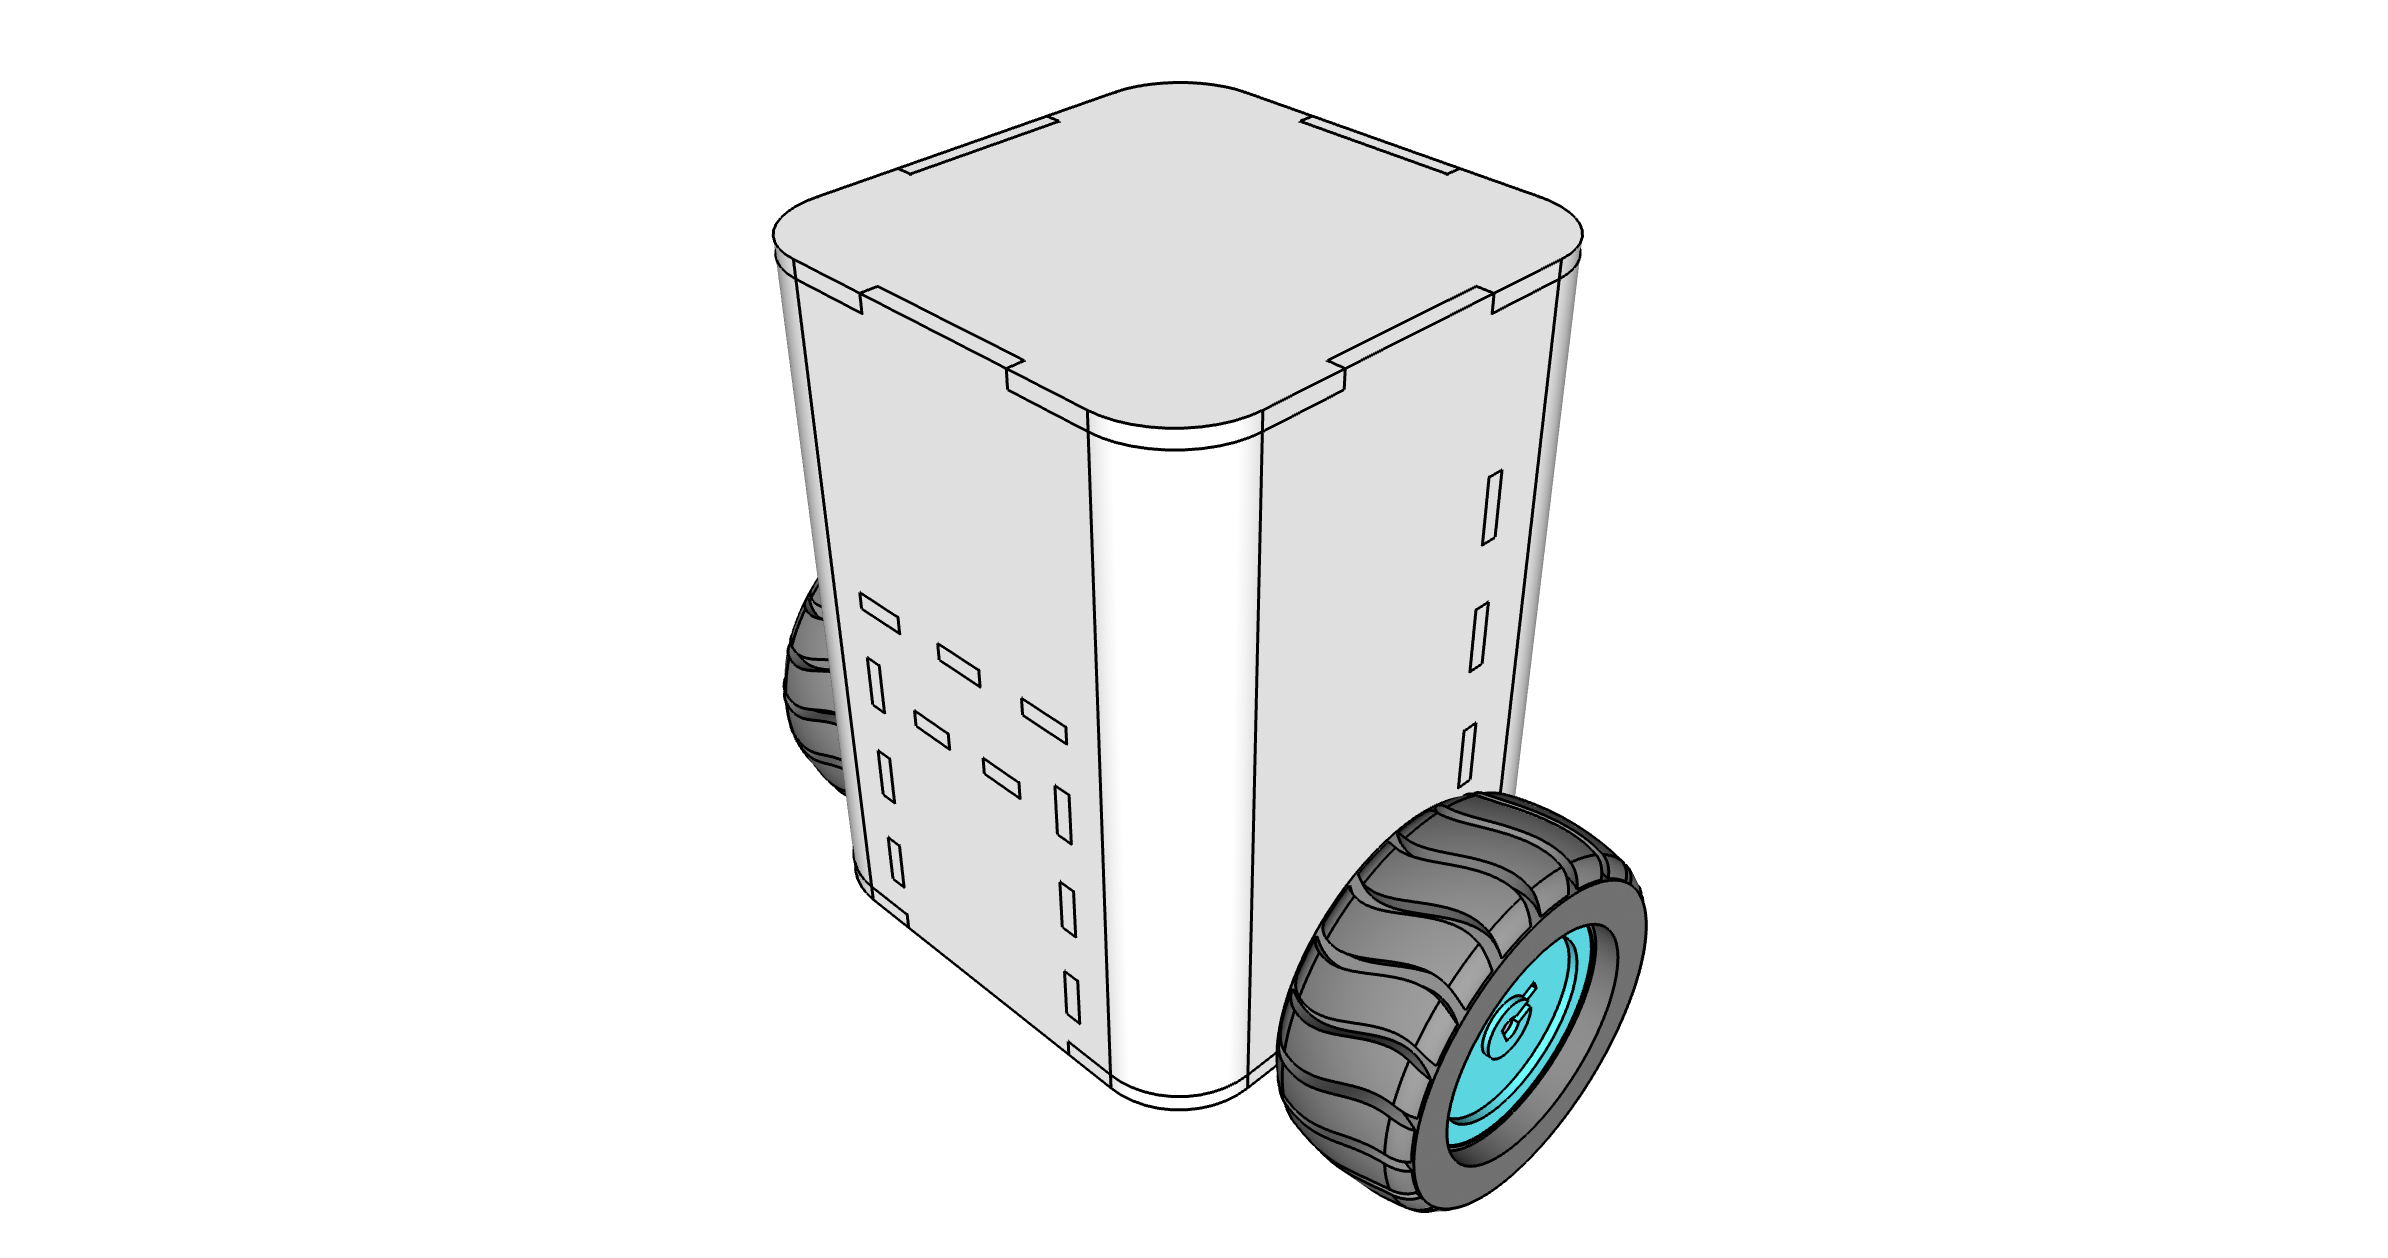
\includegraphics[width=120mm,scale=0.6]{model1.PNG}
    \caption{การออกแบบหุ่นยนต์}
    \label{fig:circuit}
\end{figure}

\subsection{แผนภาพยูสเคส (Use Case Diagram)}
\begin{figure}[ht]
    \centering
    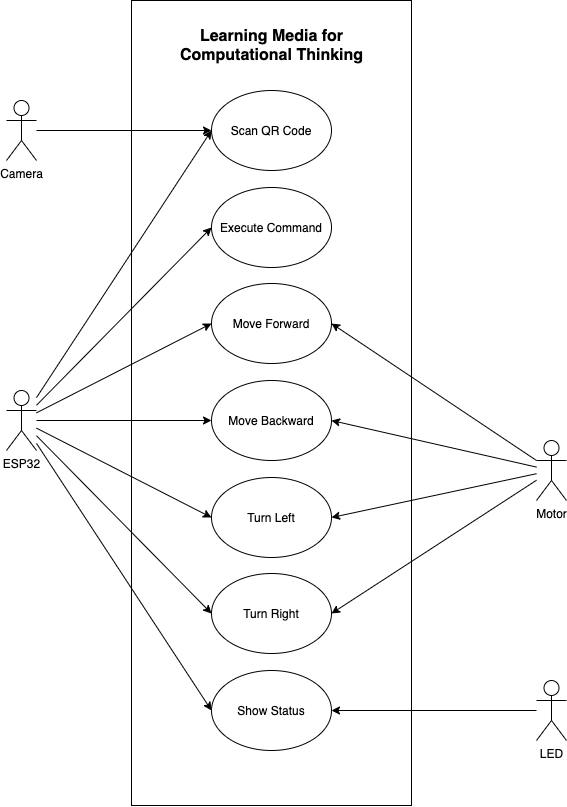
\includegraphics[width=120mm,scale=0.6]{Use_Case_Diagram.png}
    \caption{Use case diagram}
    \label{fig:Use_Case_Diagram}
\end{figure}

    \include{chapter4}
    \include{chapter5}

    \clearpage

    \def\inbib{1}
    \addcontentsline{toc}{chapter}{\bibname}
    \bibliographystyle{IEEEtran-kmitl}
    \makeatletter
    \EveryShipout{
        \ifdim\pagetotal>\pagegoal
            \if\inbib1
                \aftergroup\@cont@heading
            \else
            \fi
        \fi
    }
    \makeatother

    \bibliography{reference}
    \def\inbib{0}

    \startappendix
    \chapter{เรื่องที่หนึ่ง}


    \makeauthorbio

\end{document}
